%----------------------------------------------------------------------------------------
%	PACKAGES AND DOCUMENT CONFIGURATIONS
%----------------------------------------------------------------------------------------
\documentclass[article, a4paper, 12pt, oneside]{memoir}

% Margins
\usepackage[top=3cm,left=2cm,right=2cm,bottom=3cm]{geometry}

% Encondings
\usepackage[utf8]{inputenc}

% Language
\usepackage[portuguese]{babel}

% Graphics and images
\usepackage{graphicx}
	\graphicspath{{../images/}}

% Tables
\usepackage{tabularx}

% Paragraph Spacing
\usepackage{parskip}
\usepackage{indentfirst}
\setlength{\parskip}{0.5cm}

% Hyperreferences
\usepackage{hyperref}

% Repeated commands
\usepackage{expl3}
\ExplSyntaxOn
\cs_new_eq:NN \Repeat \prg_replicate:nn
\ExplSyntaxOff

% Header and Footer Images
\usepackage{wallpaper}

% Commands
\pagestyle{headings}

%% Linked Email
\newcommand{\email}[1]{
{\texttt{\href{mailto:#1}{#1}} }
}


%----------------------------------------------------------------------------------------
%	DOCUMENT INFORMATION
%----------------------------------------------------------------------------------------
% Title
\title{\Huge \texttt{Hospital Database (Parte 1)} }

% Authors
\author{
\LARGE \textbf{Grupo 406}\\\\
\begin{tabular}{l r}
	\email{up201806538@fe.up.pt} & Henrique Manuel Ruivo Pereira			\\
	\email{up201801011@fe.up.pt} & Iohan Xavier Sardinha Dutra Soares		\\
	\email{up201806554@fe.up.pt} & Telmo Alexandre Espirito Santo Baptista	\\
\end{tabular}
}

%\institute{Faculdade de Engenharia da Universidade do Porto \\ Bases de Dados (BDAD) - Turma 4, grupo 6}

% Date for the report
\date{\today}

% Table of Contents
\addto\captionsportuguese{\renewcommand*\contentsname{Índice}}

%----------------------------------------------------------------------------------------
%	DOCUMENT
%----------------------------------------------------------------------------------------
\begin{document}

%----------------------------------------------------------------------------------------
%	Front Page
%----------------------------------------------------------------------------------------
% Title Author and Date
\maketitle

% More information for front page
\begin{center}
\textbf{Projeto BDAD - 2019/20 - MIEIC}
\Repeat{2}{\linebreak}
\begin{tabular}{l r}
	\textbf{Professora das Aulas Laboratorias}: & Carla Alexandra Teixeira Lopes
\end{tabular}
\Repeat{4}{\linebreak}
% FEUP Logo

\includegraphics[scale=0.4]{FEUP-logo.jpg}

\end{center}

\newpage
% Header Image
\CenterWallPaper{0.1}{FEUP-logo.jpg}
\addtolength{\wpXoffset}{-7.5cm}
\addtolength{\wpYoffset}{13.8cm}

%----------------------------------------------------------------------------------------
%	ÍNDICE
%----------------------------------------------------------------------------------------
\tableofcontents*

\newpage
%----------------------------------------------------------------------------------------
%	SECTION 1 - Contexto
%----------------------------------------------------------------------------------------
\chapter[Contexto][Contexto]{Contexto}
É pretendido modelar uma base de dados para um hospital com diversos tipos de serviços disponíveis.

Sobre o próprio hospital, interessa guardar informação genérica, como o seu nome, localização completa (morada, código postal, localidade, etc), contato telefónico, bem como se o hospital é público ou privado.

O hospital é constituído por vários departamentos. Cada um destes tem nome, identificador, especializações e entidade responsável pelo departamento.

Staff, pacientes e médicos de família são pessoas, acerca das quais interessa saber o nome, o seu número de identificação único (cartão de cidadão ou equivalente), a sua morada completa (morada propriamente dita, código postal, localidade, etc), a(s) sua(s) nacionalidade(s), o seu contato telefónico, o seu número de beneficiário, o seu sexo e a sua data de nascimento.

A entidade responsável por um departamento é um membro da staff do hospital, podendo este tratar-se de um médico, enfermeiro ou técnico no hospital. Cada membro do staff tem o seu código identificador no hospital.

Especificamente sobre os médicos, é necessário guardar o número do seu consultório no hospital (caso tenha) e a sua especialização (caso tenha).
Sobre os enfermeiros, apenas é necessário guardar a sua especilização, caso a tenha.
Sobre os técnicos, apenas interessa guardar que serviço ofereçem.

Sobre os médicos de família, interessa guardar o centro de saúde ao qual está associado.

O hospital guarda informação sobre os seus pacientes como o seu grupo sanguíneo, o subsistema de saúde ao qual o paciente está associado, as doenças que o paciente tem, o seu médico de família, os médicos atribuídos naquele hospital, e as suas admissões no hospital.

Sobre cada doença interessa guardar o seu nome, uma descrição da doença e os seus sintomas predominantes.

Uma admissão no hospital tem uma data, se se trata de uma admissão de urgência e, caso seja uma urgência, a prioridade desta. Uma admissão pode desencadear vários tipos de eventos. Cada evento tem uma descrição sobre do que se trata, uma data, e outras informações dependendo do tipo de evento, que pode corresponder a: uma consulta, um exame, uma intervenção ou um internamento.

Numa consulta, interessa guardar o médico que a realizou e o diagnóstico da consulta.\\
Num exame, guarda-se o nome do exame feito e uma descrição deste.\\
Numa intervenção, guarda-se uma descrição da intervenção realizada.
Num internamento é necessário guardar o quarto onde o paciente se encontra, o motivo do internamento e a data na qual o paciente recebeu alta (saiu do internamento) caso tal já tenha acontecido.

\newpage
%----------------------------------------------------------------------------------------
%	SECTION 2 - UML
%----------------------------------------------------------------------------------------
\chapter[UML - Modelo Conceptual][UML]{UML - Modelo Conceptual}
\begin{center}
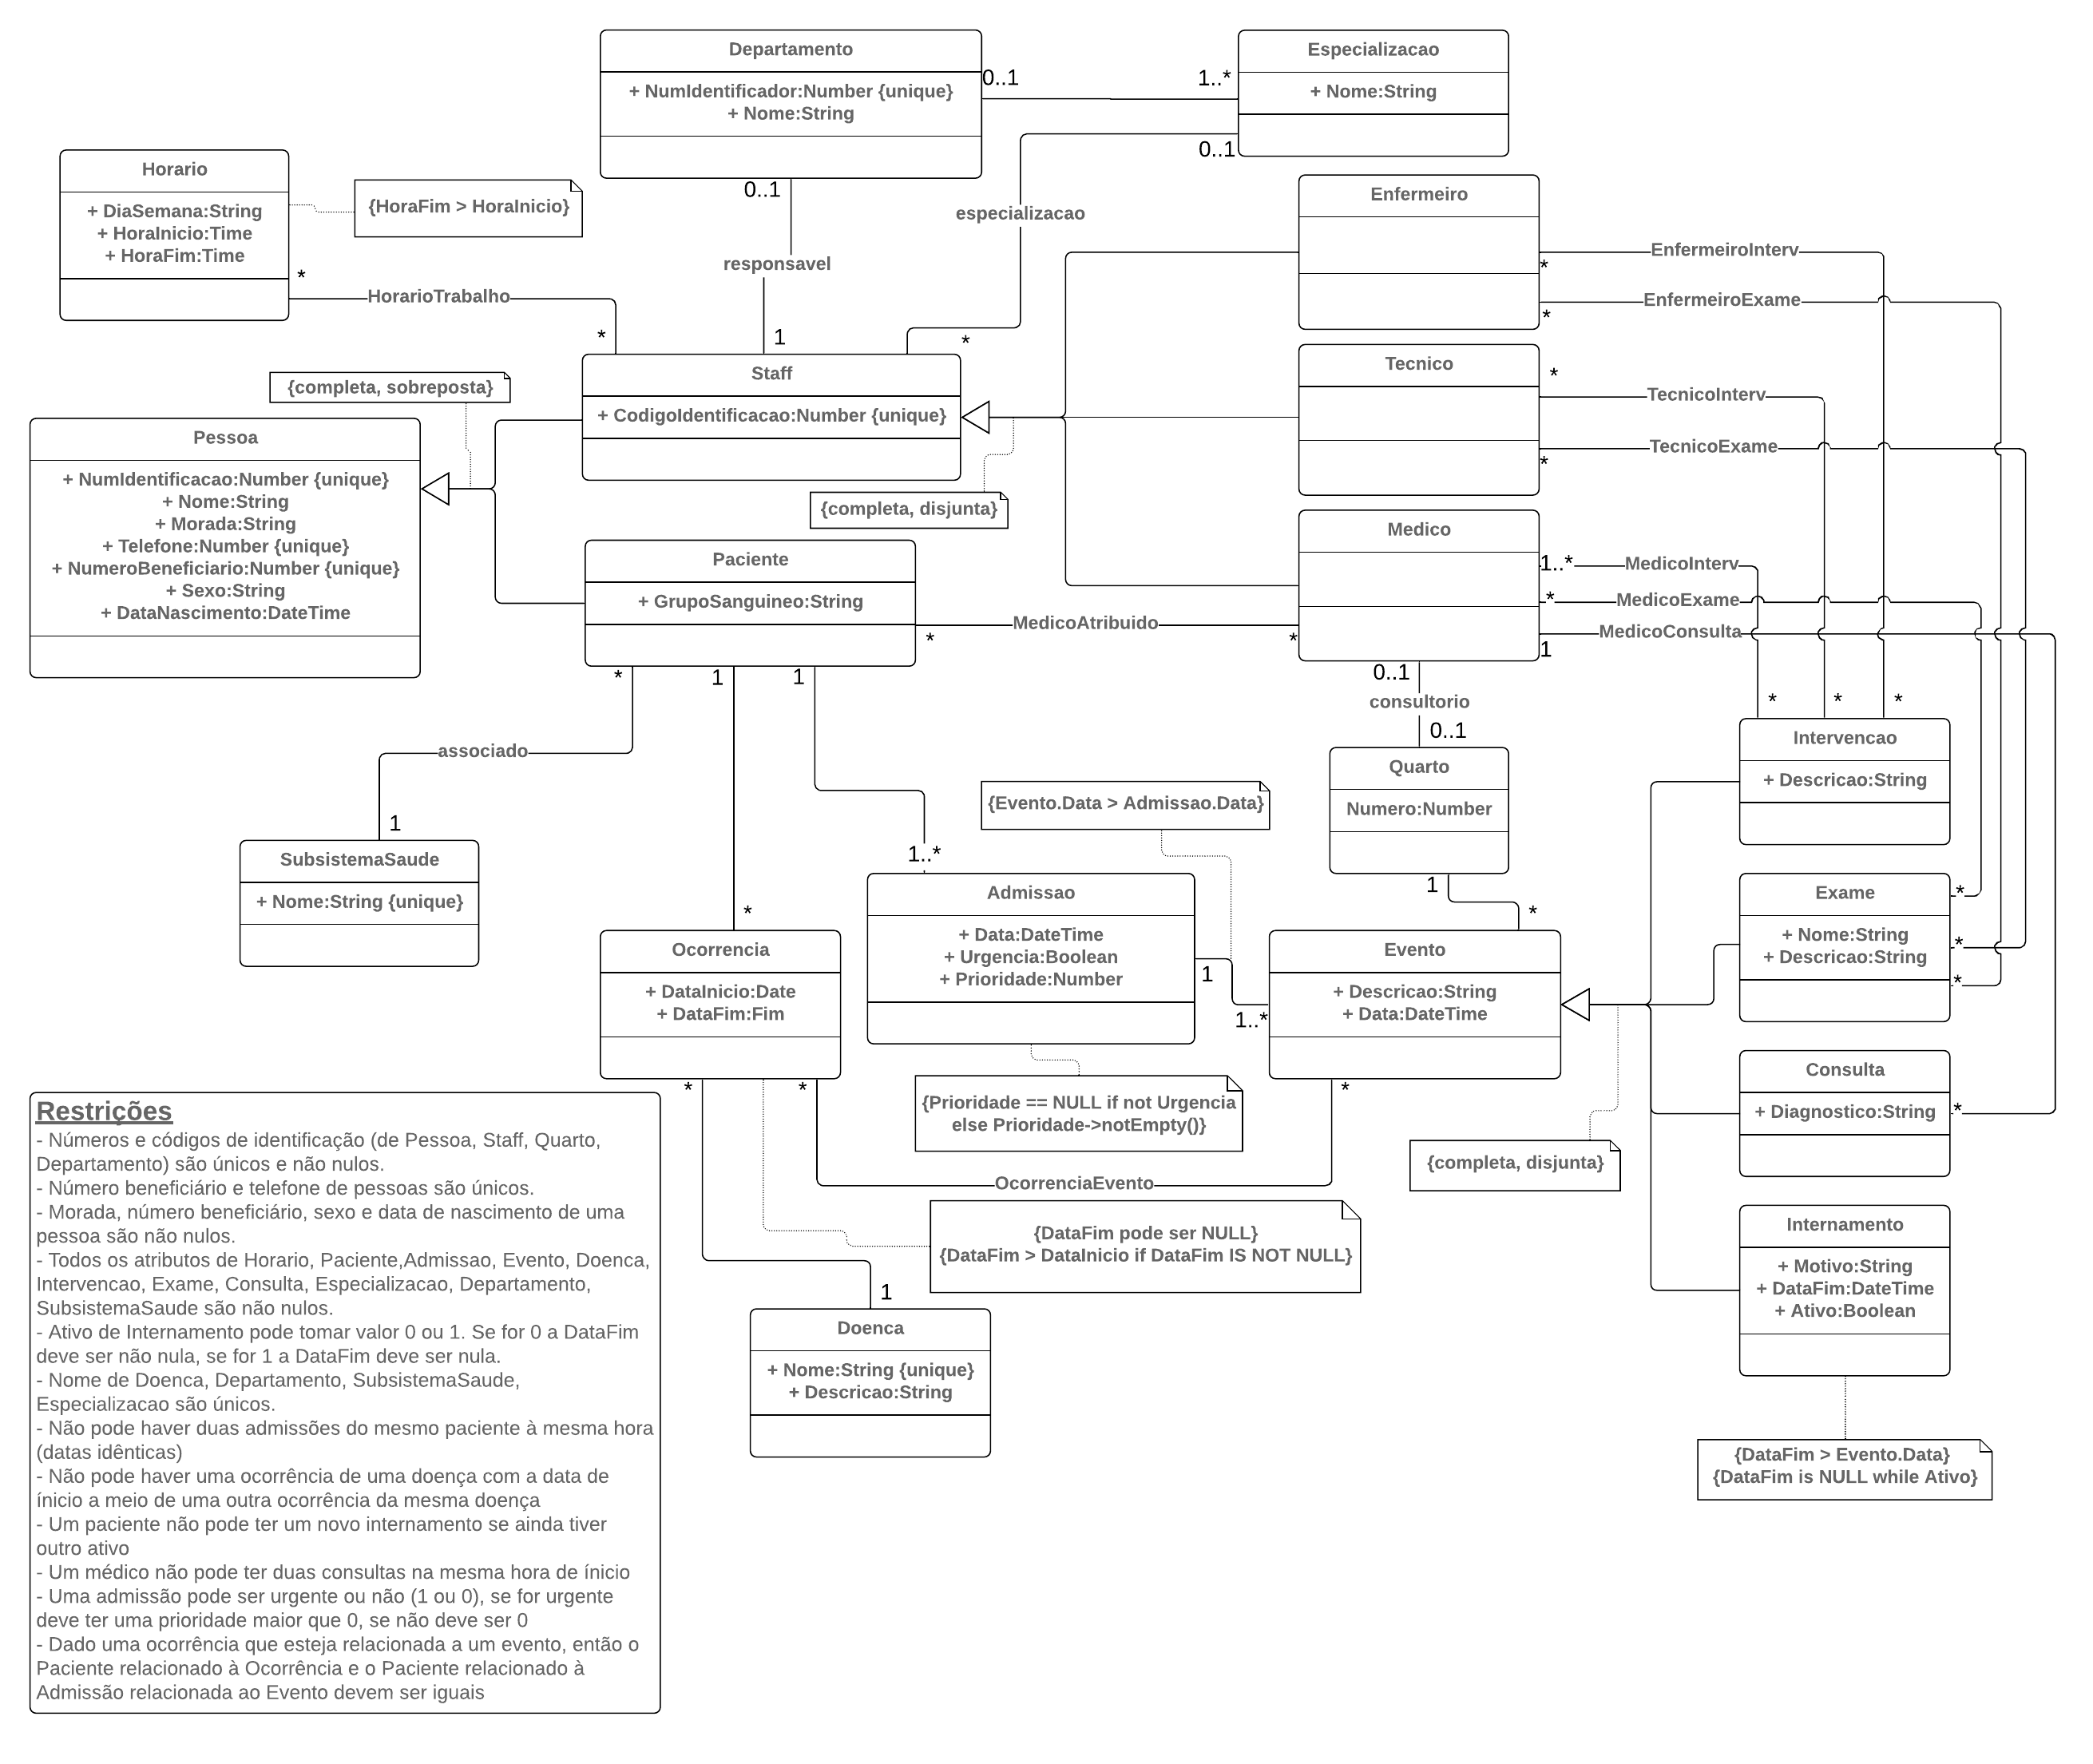
\includegraphics[width=1.0\linewidth, height=1.0\linewidth]{BDAD-UML.png}
\end{center}

\end{document}
